\def\year{2019}\relax
%File: formatting-instruction.tex
\documentclass[letterpaper]{article} %DO NOT CHANGE THIS
\usepackage{aaai19}  %Required
\usepackage{times}  %Required
\usepackage{helvet}  %Required
\usepackage{courier}  %Required
\usepackage{url}  %Required
\usepackage{graphicx}  %Required
\frenchspacing  %Required
\setlength{\pdfpagewidth}{8.5in}  %Required
\setlength{\pdfpageheight}{11in}  %Required
%PDF Info Is Required:
\pdfinfo{
	/Title (2019 Formatting Instructions for Authors Using LaTeX)
	/Author (AAAI Press Staff)}
\setcounter{secnumdepth}{0}  

\newtheorem{theorem}{Theorem}
\newtheorem{definition}{Definition}
\newtheorem{lemma}{Lemma}
\newenvironment{proof}{{\noindent\it Proof}\quad}{\hfill $\blacksquare$\par}
\usepackage{amsmath,amssymb,amsfonts}
\usepackage{mathrsfs,algorithm,algorithmicx,algpseudocode}
\usepackage{diagbox}



\begin{document}


% The file aaai.sty is the style file for AAAI Press 
% proceedings, working notes, and technical reports.
%
%\begin{frontmatter}
\title{Scale-Clip Net: Shape Distribution For Low-Bit Quantization}
\author{ID: 6210
}


\maketitle
\begin{abstract}
Quantization, as an effective strategy for reducing computational cost of deep neural network, has promoted the deployment of the network into computation source-limited devices. Most conventional quantization methods just focus on minimizing the loss between the float point model and quantized model, without considering the relationship between distribution and quantization. In this paper, we turn to exploring what kind of distribution of float point model is good for quantization. We first introduced a quantitative metric to measure the quantized loss ratio (QLR) and experimentally found that small QLR is especially suited for low-bits quantization, which can recover the lost accuracy easily by fine-tuning. Theoretically we proved that the distribution with small ratio of {\it abs-max} to {\it abs-mean} leads to small QLR. Based on above theory, we proposed a Scale-Clip method, which clips the outliers of weight and activation with the dynamic threshold, shaping weight and activation into a distribution suited for quantization. With incorporating Scale-Clip method into quantization framework, we perform experiments on the image classification, object detection and semantic segmentation tasks and demonstrate that the proposed method achieves much better performance than the state-of-the-art quantization methods.


\end{abstract}

\section{Introduction}
In recent years, convolutional neural network(CNN) has helped Computer Vision get significant breakthroughs in variety of tasks, 
such as image classification, object detection, semantic segmentation, etc.
However, these deep networks contain millions of learnable weights,leading to the drastically increasing in computation source cost and test-phase time,
which critically restricts the deployment of models in limited computation resources devices with ARM or FPGA. To alleviate this problem, several methods have been developed, such as 
designing computational efficient networks~\cite{howard2017mobilenets,hluchyj1991shuffle},
pruning the network with less channels and sparser weights\cite{he2017channel,liu2017learning}, etc.
% distilling the small network from big network with co-training,
Among the existing approaches, quantization has attracted great attention in recent years 
for its capability of saving computation resources 
and facilitating the deployment of complex model into computation source-limited devices. Moreover, low-bit fixed point quantization has great advantage in reducing storage and computation complexity. It not only replaces the expensive full precision multiplication in regular convolution with low bit multiplication, which can be further simplified by bit shifting. Hence it is worthwhile to investigate into low bit model quantization.
% Quantization mainly means discretizing weights or activations of full precision(i.e., 32-bit floating-point) into low-bit fixed point number
% without modifying the model architecture, 
% so that each weight(or activation) can be represented by fewer bits. 
% For example, if weights only take on 16, then each weight could be encoded in 4 bits.
In order to obtain low-bit models, previous works have largely been carried out in two aspects. 
One aspect is to improve the method of training quantized model. 
The other aspect is to explore the proper quantization strategy.

For the training method, there have established some common frameworks for training arbitrary low-bit model, 
such as DoReFa-Net~\cite{zhou2016dorefa} and Ristretto~\cite{gysel2016ristretto}. 
Furthermore, TWN~\cite{zhu2016trained} attempts to use ternary values to represent weights and achieves promising performance on ImageNet~\cite{deng2009imagenet}, without quantizing activations. XNOR-Net~\cite{rastegari2016xnor} and BNN~\cite{courbariaux2016binarized} propose training method which allows simultaneously quantizing the network weights and activations into binary values.
INQ~\cite{zhou2017incremental} and ELQ~\cite{zhou2018explicit} adopts incremental strategy that fixes some part of weights and updates the rest to compensate the degradation of performance.  
\cite{mishra2017apprentice,polino2018model} introduce model distillation into quantization schemes, training the low-bit model in the guidance of full precision model.
TSQ~\cite{wang2018two} decouples the weight and activation quantization and proposes a two-stage training method.
\begin{figure*}[ht!]
	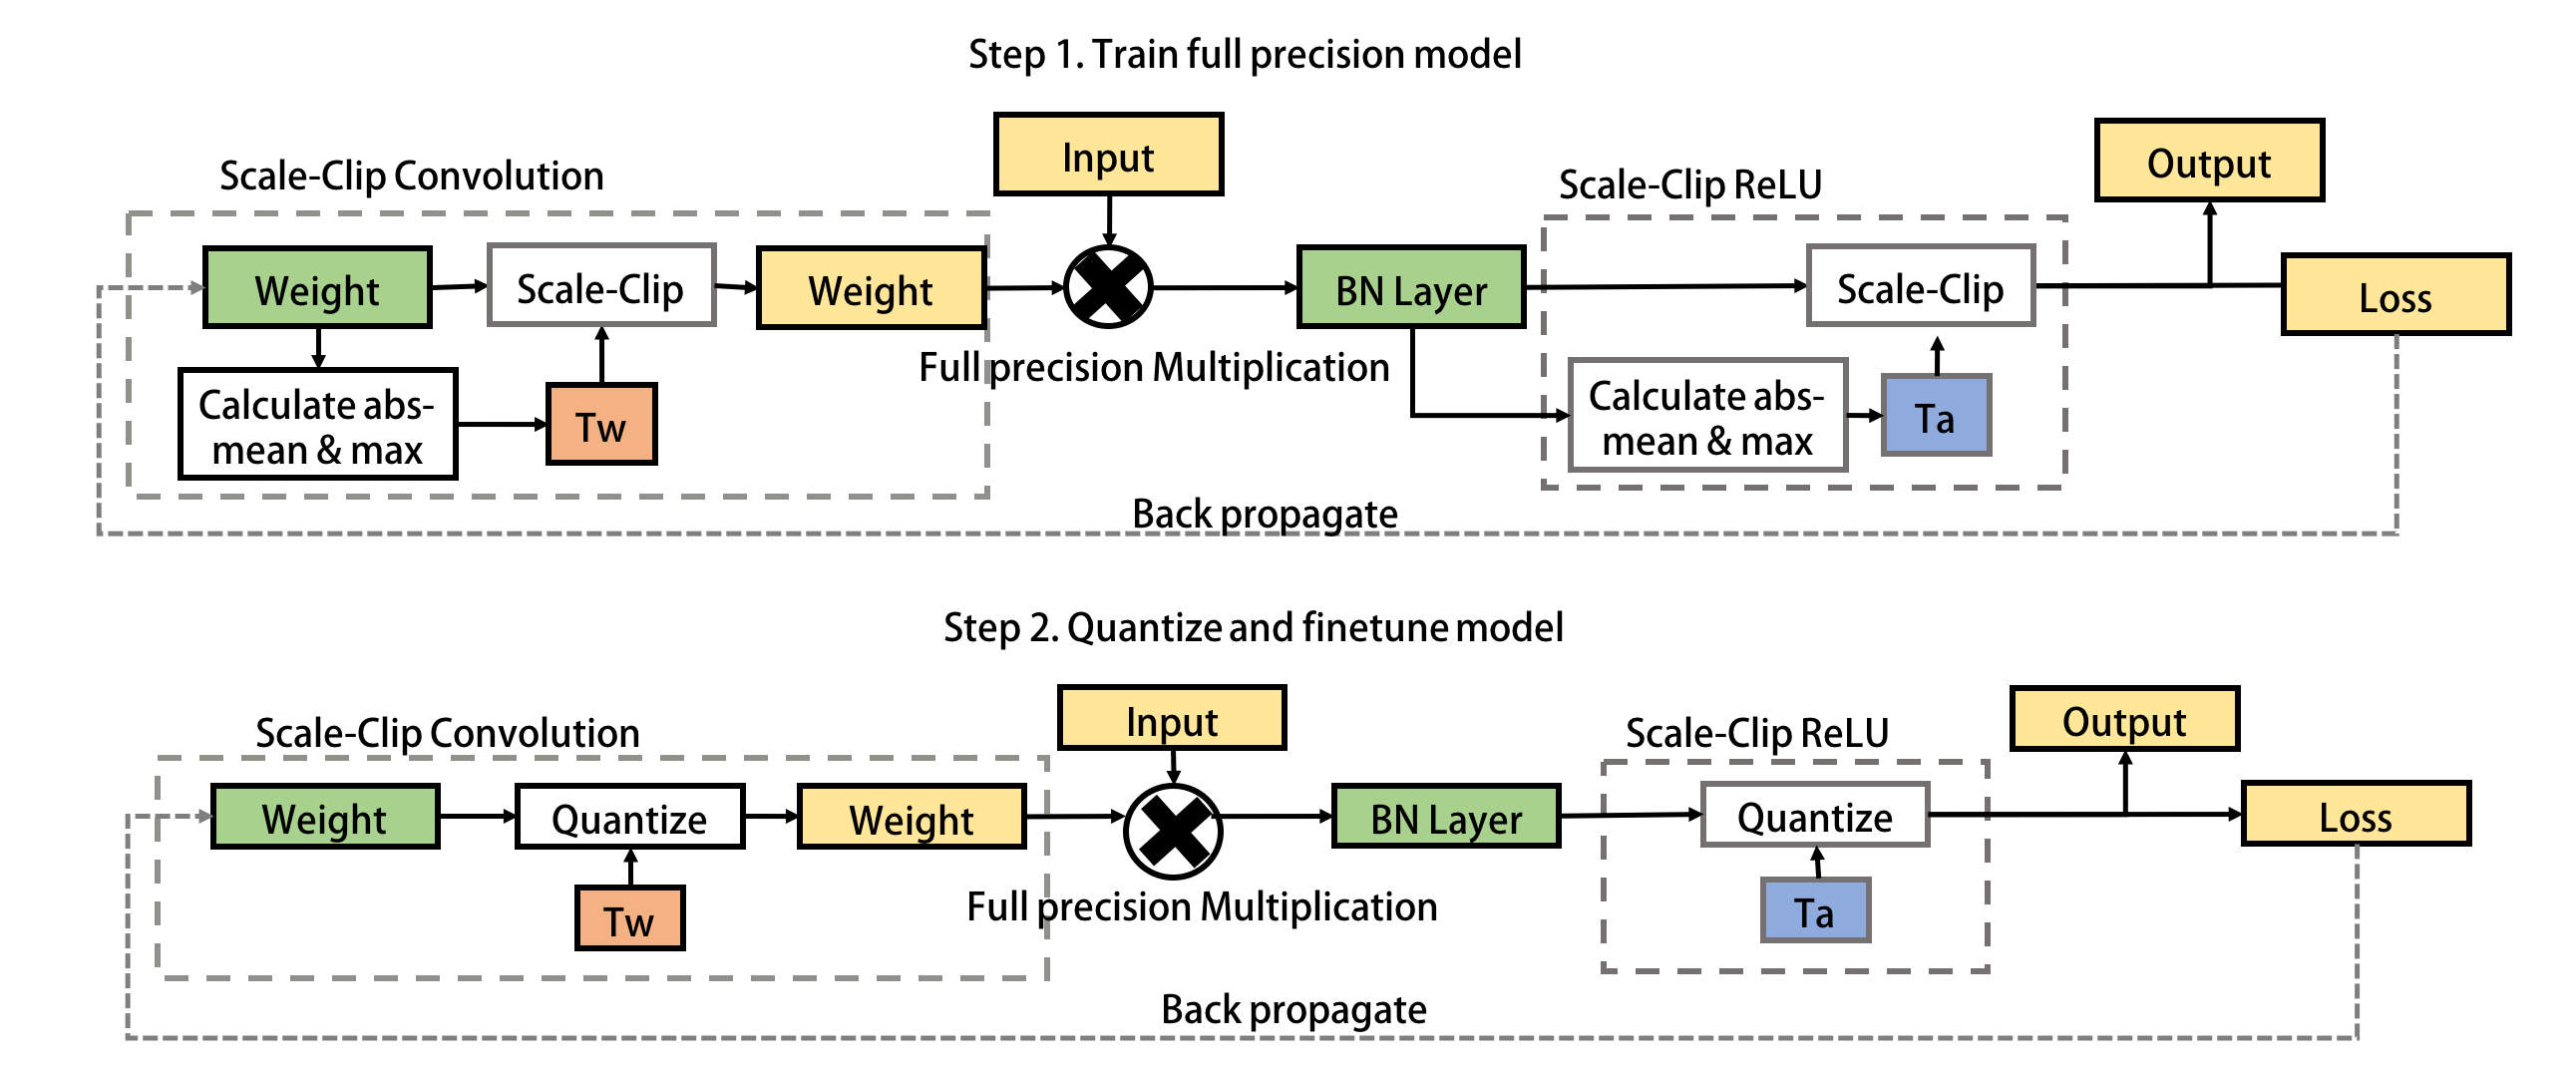
\includegraphics[width=1.0\textwidth]{quantization_framework.png}\label{training-quantization-framework}
	\caption{Training framework. In the Step 1, we train the full-precision model. We substitute the all convolution and ReLU layers with our Scale-Clip version, and adopt Algorithm \ref{alg:1} to update the network. In the Step 2, we analyze the statics of weight and activation, then quantize the full-precision model into low-bit fixed-point model. We adopt the uniform quantization scheme and quantize the whole network simultaneously. In the Step 3, we finetune the quantized model. We adopt the mentioned previous work, which forward propagate with fixed-point number, but back propagate the gradient on the full-precision number.}
\end{figure*}

\begin{figure*}[ht!]
	\centering
	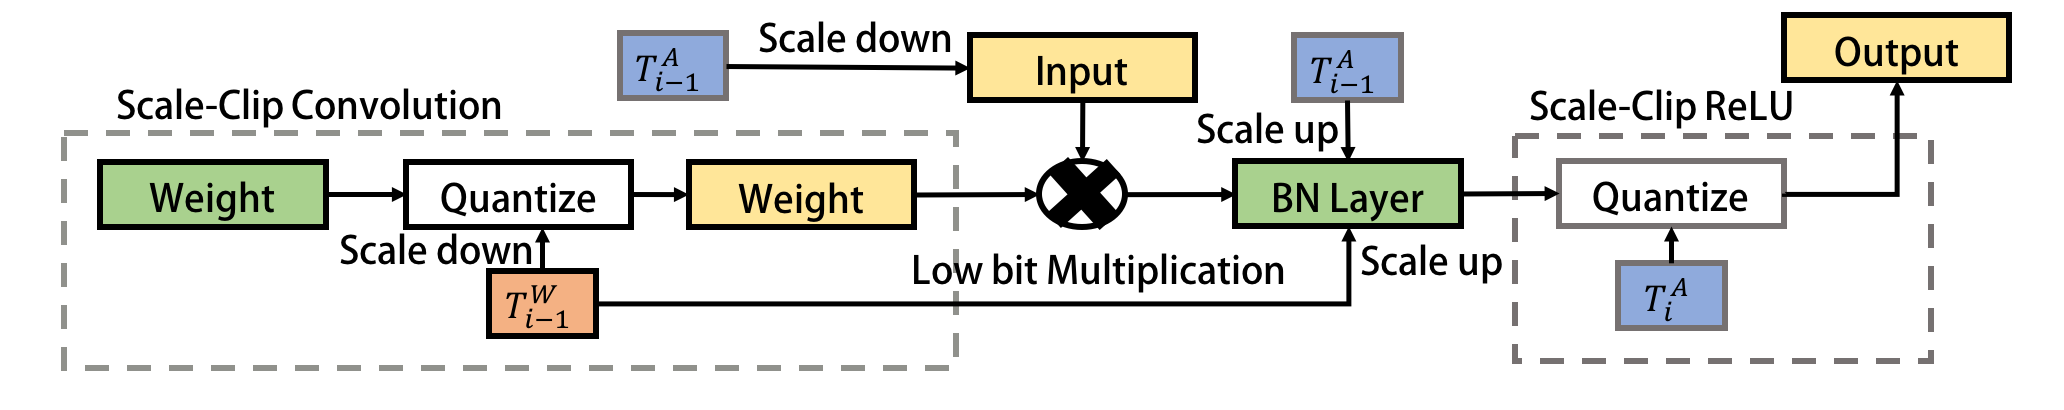
\includegraphics[width=0.8\textwidth]{inference_framework.png}
	\caption{Inference framework. When quantizing the input and weight, we first scale down the input and weight into $[0, 2^m-1]$ and $[0,2^n-1]$ by multiplying $\frac{2^m-1}{T^W_{i}}$ and $\frac{2^n-1}{T^A_{i-1}}$, then quantize the weights and input data using uniform quantization scheme. Notice that we merge the $\frac{2^m-1}{T^W_{i}}$ and $\frac{2^n-1}{T^A_{i-1}}$ into Batch normalization layer for computation simplicity. The output data is quantized after Batch Normalization.}\label{inference framework}
% 	Afterwards, we quantize the input and weight, and implement the convolution operation with $m+n+\lceil log_2(kernel\_size^{2})\rceil+1$ bit number. The threshold of Scale-Clip ReLU is $[0,T^{A}_{i}]$. 
\end{figure*}
For quantization strategy, one way is to optimize the quantization levels. To determine the quantization levels, some work fully analyze the distribution of weights and activations of full precision model. 
BalanceQ~\cite{zhou2017balanced} selects the quantization bins with Histogram Equalization.
~\cite{park2017weighted} determines the quantization levels by maximizing the weighted entropy.
% Some work also use the low rank matrix approximation~\cite{denton2014exploiting,jaderberg2014speeding,kim2015compression}, 
% or cast weights into optimal quantization levels to minimize the reconstruction error~\cite{}. 
FFN\cite{wang2017fixed} approximate the weight matrix by the weighted sum of outer product of several vector pairs with ternary entries vectors. 
Other work attempt to change the distribution of activation functions. 
HWGQ\cite{cai2017deep} introduces clipped and log-tailed ReLU versions to remove outliers and utilizes Half Wave Gaussian Quantizer to quantize the activations. PACT\cite{choi2018pact} squeezes the dynamic range of the activations by a learnable upper bound, resulting in a more robust quantization performance.

Despite of tremendous advances of above methods, 
there is still a key point people may overlook: what distribution is proper for quantization? In this paper, inspired by the phenomenon we observed in engineering that different distribution of full precision models lead to different quantization performance, we will explore what distribution of the full precision model is easy to quantize, and furthermore attempt to shape the distribution into the specific distribution.

\begin{figure}[ht!]
	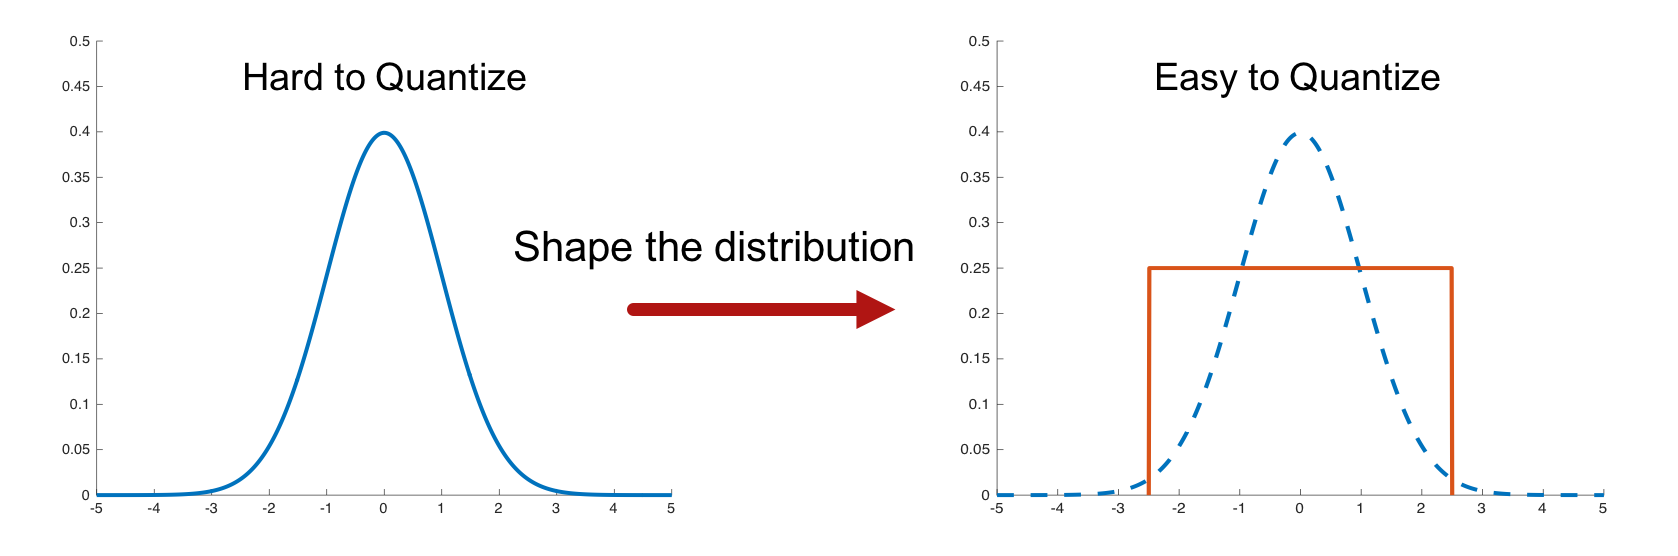
\includegraphics[width=0.45\textwidth]{gaussian-uniform.png}
	\caption{Original distribution of weight is hard to quantize, since the outliers impair the quantization precision. We shape the distribution of weights and make it easier to quantize the network.}\label{fig:gaussian}
\end{figure}
We start with the definition of \textbf{Q}uantization \textbf{L}oss \textbf{R}atio(QLR), 
which is similar to Signal Noise Ratio(SNR) and could measure the signal loss after quantization.
To simplify the discussion, we only consider weight quantization with activation staying as full precision. 
The empirical idea is that the smaller the QLR is, 
the more easily can quantized model recover the lost accuracy by finetuning.
To minimize QLR, we find that the weight distribution with small ratio of abs-max to abs-mean holds smaller QLR.
The theory is proved by computing the expectation of quantization loss as an intermediate proof.

Based on above theory, we attempt to explore how to train the full precision model to the specific distribution while ensuring high performance.
We propose an effective method called \emph{Scale-Clip}, which determines the threshold by the weight's average energy and clips the outliers.
Afterwards, we generalize the Scale-Clip method to quantizing activations by transforming the vanilla ReLU into Scale-Clip ReLU. In the end, we apply the Scale-Clip method for weights and activations to our quantization framework to get the final low-bit fixed point model. The overview of our quantization framework is presented in Fig~\ref{training-quantization-framework} and Fig~\ref{inference framework}. 
We evaluate our method on many experiments such as ImageNet classification task and Cityscape segmentation task.
The results show that our framework outperforms than other state-of-the-art methods.

The main contributions of this paper lie in the followings:
\begin{enumerate}
	\item We find and prove that the distribution with small ratio of abs-max to abs-mean is more suitable for quantization.
	\item We propose an effective Scale-Clip method to shape the distribution of full precision model into flatter distribution while ensuring high performance.
	\item We apply the Scale-Clip method into the quantization framework, and validate that our method outperforms than state-of-art methods in variety of tasks such as ImageNet Classification task.
\end{enumerate}

% \section{Preliminary}\

% Before introducing our work, we give some preliminaries to help understand our works.

% \subsection{Dynamic Fixed Point Quantization}
% The different layers' weight of $\mathbf{CNN}$ model have different range.
% Fixed point may have no capacity to cover these range, but dynamic fixed point could overcome this problem.

% For a dynamic fixed point number $w$, it could be represented as
% \begin{equation}
% w=(-1)^{s}\cdot 2^{WL-IL-1}\sum_{i=0}^{B-2}2^{i}\cdot x_{i}
% \end{equation}
% where $B$ denotes the total bit-width, $s$ is the sign bit, $IL$ is the
% integral length which can be negative and $x$ is the mantissa bits. 

% For a given layer's weight $\mathbf{W}_{i}$ of float point model, 
% the required integral length $IL$ could be computed as
% \begin{equation}
% IL=\lfloor lg_{2} (\max_{w\in \mathbf{W}_{i}}|w|+1)\rceil
% \end{equation}
% Therefore, the range of the $\mathbf{W}_{i}$ is related to $2^{IL}$.
% \subsection{Quantization Inference}
% In our work, we choose the quantization inference framework that compute the multiplication in full precision.
% The inference framework is composed of: quantizing the weight and input, computing the convolution in float point model, then quantizing the output. It is also performed in Fig \ref{inference framework}
% \begin{figure}[ht!]
% 	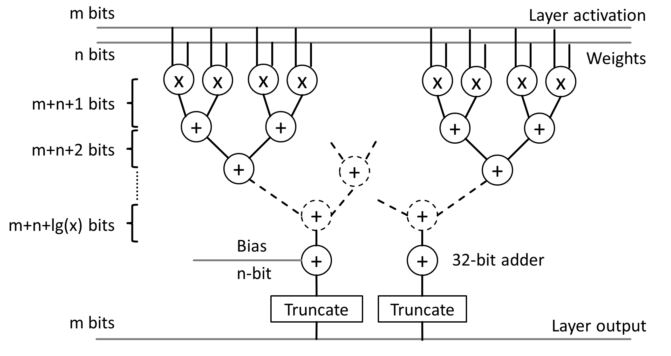
\includegraphics[width=0.45\textwidth]{inference_framework.jpg}
% 	\caption{Inference Framwork}\label{inference framework}
% \end{figure}

\section{Scale-Clip Net}
In this section, we propose a Scale-Clip method to reshape the distribution of full precision model's weights and activations for better quantization performance.
We first state what distribution is good for quantization;
then we design an effective algorithm to implement the Scale-Clip method.

Before all, we roughly explain our quantization training and inference framework to get low-bit fixed point model.
The training framework is composed of two steps: training a full precision model with Scale-Clip method and 
fine tuning the quantized model to recover the lost accuracy.
For fine tuning, we adopt the training scheme mentioned in \cite{gysel2016ristretto,polino2018model}, which forward propagates with fixed point weights, but back propagates the full precision gradient and update the full precision weights.
The training framework is also displayed in Fig \ref{training-quantization-framework}.
The core of our quantization inference framework is operating the quantized the weight and input in full precision number, 
which is performed in Fig \ref{inference framework}.

\subsection{Distribution Exploration}
If we regard trained CNN as a nonliner regressor, then it could be denoted as 
\begin{equation}
f^{*}=f(\mathbf{x};\mathbf{W}_1,\mathbf{W}_2\dots,\mathbf{W}_m)
\end{equation}
where $\mathbf{x}$ is the input of CNN, $\mathbf{W}_{i}$ is the $i$th convolution layer's weight of trained model,
and $\mathbf{W}_{i}=\{w_{ij},j=1\cdots,n_i\}$.
We denote $\mathbf{I}_i$ as the input of $i$th convolution layer, $\mathbf{O}_i$ as the output of $i$th convolution layer,
then $\mathbf{O}_i=\mathbf{I}_i\otimes \mathbf{W}_i$.

To simplify the discussion, we consider a model with quantized weights $\mathbf{W}_{i}$
in following form
\begin{equation}
\tilde{f}^{*}=f(\mathbf{x};\tilde{\mathbf{W}}_1,\tilde{\mathbf{W}}_2\dots,\tilde{\mathbf{W}}_m)
\end{equation},
where $\tilde{\mathbf{W}}_{i}$ is denoted as quantized $\mathbf{W}_{i}$, then $\tilde{\mathbf{O}}_i=\mathbf{I}_i\otimes \tilde{\mathbf{W}}_i$. 
According to the linear property of convolution, we have 
\begin{equation}
	\begin{aligned}
	\Delta \mathbf{O}_{i} &=\mathbf{O}_i-\tilde{\mathbf{O}}_i\\
	&=\mathbf{I}_i \otimes \mathbf{W}_i-\mathbf{I}_i\otimes \tilde{\mathbf{W}}_i\\
	&=\mathbf{I}_i\otimes(\mathbf{W}_{i}-\tilde{\mathbf{W}}_i)\\
	&=\mathbf{I}_i\otimes \Delta \mathbf{W}_{i}
	\end{aligned}
\end{equation}

Since the signal propagates through layer by layer, similar to $\mathbf{SNR}$(signal noise ratio), 
we have 
\begin{equation}
\mathbf{SNR}_i=\frac{||\Delta \mathbf{O}_{i}||_F^2}{||\mathbf{O}_i||_F^2}
\end{equation}
Due to the powerful capacity of CNN, there are numerous regressors with different weight distribution that can achieve high performance. So here comes up an intuitive idea:
a model with small quantization $\mathbf{SNR}$ will largely maintain its performance after quantization, and can also easily retrieve its performance by finetuning.

Suppose the input data can be modeled as a Gaussian Distribution $\mathcal N(0, \sigma^2)$. According to \emph{Parseval} Theorem, 
\begin{equation}
    \begin{aligned}	
    \mathbf{SNR}_i
	& = \frac{||\mathbf{I_i} \otimes \Delta \mathbf{W}_{i}||_F^2}{|\mathbf{I_i} \otimes {\mathbf{W_i}}||_F^2} \\
    & = \frac{||\mathcal{F}(\mathbf{I_i})\mathcal{F}(\Delta \mathbf{W}_{i})||_F^2}{||\mathcal{F} (\mathbf{I_i})\mathcal{F}({\mathbf{W_i}})||_F^2} \\
%     & = n_q^2\frac{||\mathcal{F}(\mathbf{I_i})||^2_2}{||\mathcal{F} (\mathbf{I_i})\mathcal{F}({\mathbf{W_i}})||_2^2} \\
%     & \ge n_q^2\frac{||\mathcal{F}(\mathbf{I_i})||^2_2}{||\mathcal{F} (\mathbf{I_i})||_2^2||\mathcal{F}({\mathbf{W_i}})||_2^2} \\
    & = \frac{||\Delta \mathbf{W}_{i}||_F^2}{||\mathbf{W_i}||_F^2} \\
    & = \frac{\mathbb{E}(\Delta \mathbf{W}^2_{i})}{\mathbb{E}|\mathbf{W_i}^2|} \\
    & \le \frac{\mathbb{E}(\Delta \mathbf{W}^2_{i})}{\mathbb{E}^2|\mathbf{W_i}|} = \mathbf{QLR}_i^2
    \end{aligned}
\end{equation}.
% To bridge the $\mathbf{SNR}_i$ with the weight distribution, 
where we denote \textbf{Q}uantization \textbf{L}oss \textbf{R}atio ($\mathbf{QLR}_{i}$) as:
\begin{equation}
\mathbf{QLR}_{i}=\frac{\mathbb{E}^{\frac{1}{2}}(\Delta \mathbf{W}_{i})}{\mathbb{E}|\mathbf{W_i}|} 
\end{equation}
Hence we convert optimizing the $\mathbf{SNR}_i$ into optimizing its upper bound $\mathbf{QLR}_{i}^{2}$, which is more simple for calculation and analysis. We firstly propose Theorem \ref{the:range-mean} to optimize $\mathbf{QLR}_{i}$.

\begin{theorem}\label{the:range-mean}
	Suppose that $\mathbf{W}_{i}$ are quantized into $n$ bits, $\mathbf{QLR}_{i}$ $\propto$ $\frac{\max|\mathbf{W}_i|}{\mathbb{E}{|\mathbf{W}_{i}|}}$.
\end{theorem}
\begin{proof}
	Denote $\max|\mathbf{W}_i|$ as $\alpha$. Using the uniform quantization scheme,
	\begin{equation}
    \tilde{\mathbf{W}_{i}}=round(\tilde{\mathbf{W}_{i}} \cdot \frac{2^{n-1}-1}{\alpha}) \cdot \frac{\alpha}{2^{n-1}-1}
	\end{equation}
then $\mathbf{W}_i$ can be rewritten as the sum of quantized value and quantization error $\Delta \mathbf{W}_{i}$.
	\begin{equation}
	\mathbf{W}_{i}=\tilde{\mathbf{W}_{i}}+\Delta \mathbf{W}_{i}
	\end{equation}
	where $\Delta \mathbf{W}_{i} = \mathbf{n}_{i}\frac{\alpha}{2^{n-1}-1}, \mathbf{n}_{i} \in [-\frac{1}{2},\frac{1}{2})$. We denote $\mathbb{E}(\mathbf{n}^2_{i})$ as $n^2_q$, which is exactly the variance when $n_q$ has zero mean. Then $\mathbb{E}^{\frac{1}{2}}(\Delta \mathbf{W}_{i})$ can be further written as
	\begin{equation}
	\begin{aligned}
	\mathbb{E}(\Delta \mathbf{W}_{i})
	&=\frac{\alpha}{2^{n-1}-1}\mathbb{E}^{\frac{1}{2}}(\mathbf{n}_{i}^2) \\
	&=\frac{\alpha n_{q}}{2^{n-1}-1} \\
	\end{aligned}
	\end{equation}
So it can be drawn out that
	\begin{equation}
	\mathbf{QLR}_{i} = \frac{\mathbb{E}^{\frac{1}{2}}(\Delta \mathbf{W}_{i})}{\mathbb{E}|\mathbf{W}_i|} = \frac{\alpha}{\mathbb{E}|\mathbf{W}_i|} \cdot \frac{ n_{q}}{2^{n-1}-1}
	\end{equation}
% 	Since there are $n_{i}$ (usually very large) weights in $\mathbf{W}_{i}$, the sum of quantization error can be approximated by the sum of their expectations as below.
% 	\begin{equation}
% 	\begin{aligned}
% 	\frac{\sum_{j}|w_{ij}-\tilde{w}_{ij}|}{\sum_{j}|w_{ij}|}
% 	&=\frac{n_{i}E(|w_{ij}-\tilde{w}_{ij}|)}{n_{i}|\overline{\mathbf{W}_{i}}|}\\
% 	&=\frac{\alpha}{|\overline{\mathbf{W}_{i}}|} \cdot \frac{n_{q}}{2^{n-1}-1}
% 	\end{aligned}
% 	\end{equation}
	Furthermore, the quantization variance $n_q^2$ is independent to weights,
	hence we have that $\mathbf{QLR}$ is proportion to the $\frac{\max(|\mathbf{W}_i|)}{\mathbb{E}(|\mathbf{W}_{i}|)}$.
\end{proof}

\subsection{Scale-Clip Method}\

To get a better quantized model, we should restrict the weight distribution to get ratio as small as possible:
\begin{equation}\label{qwlr_argmin}
\begin{aligned}
	& \min_{\mathbf{W}_{i}} \mathbf{QLR}\\
	 s.t. \\
	 & \mathbf{y}=f(\mathbf{x};\mathbf{W}_1,\mathbf{W}_2\dots,\mathbf{W}_m)
\end{aligned}
\end{equation} 
Based on Theorem \ref{the:range-mean}, the (\ref{qwlr_argmin}) is equivalent to the following form:
\begin{equation}\label{equ:max-mean}
\begin{aligned}
& \min_{\mathbf{W}_{i}} \frac{\max|\mathbf{W}_i|}{\mathbb{E}|\mathbf{W}_i|},i=1,\cdots,m \\
s.t. \\
& \mathbf{y}=f(\mathbf{x};\mathbf{W}_1,\mathbf{W}_2\dots,\mathbf{W}_m)
\end{aligned}
\end{equation} 

However, it is difficult to directly solve (\ref{equ:max-mean}).
Instead, we propose an effective Scale-Clip method to restrict the distribution of weights and activations of the full precision model.
For weights, Scale-Clip method is to clip weights with the dynamic threshold relied on the average energy of weights. One simple form is defined as:
\begin{equation}
Q(w)=\left\{
   \begin{array}{lr}
      T^w_i, & w \ge T^w_i \\
      w, & w \in (-T^w_i, T^w_i) \\
      -T^w_i, & w \le -T^w_i 
   \end{array}
\right.
\end{equation}
\begin{equation}\label{threshold}
	T^w=k \cdot \mathbb{E}|\mathbf{W}_{i}|
\end{equation}
where $k$ is called Scale-Clip factor which needs to be set specifically. 

% When weights hit the clipping threshold $\alpha$, they keep still at the boundary, which is called direct clipping. 

% The relationship between $\frac{\max{|\mathbf{W}_i|}}{\overline{|\mathbf{W}_{i}|}}$ and the distribution of weights is usually complex. We choose three common distributions to discuss the their relationships.

% \paragraph{Bernoulli Distribution} Suppose $X \in B(1,p)$, and the value of X can be either $-\max|\mathbf{W}_{i}|$ or $\max|\mathbf{W}_{i}|$. In this case, the Bernoulli distribution is equivalent to $k=1$ since all the absolute value of weights are the same. In other words, if we set $k=1$, we actually train a binary network. 

% \paragraph{Uniform Distribution} Suppose $X \in U(-a,a)$, where $a=\max(|\mathbf{W}_{i}|)$. It can be obtained that $\overline{|\mathbf{W}_{i}|}$ equals to $\frac{1}{2}\max(|\mathbf{W}_{i}|)$, which means $k=2$. But the Uniform distribution cannot be interpreted by $k=2$.

% \paragraph{Gaussian Distribution} Suppose $X \in N(0,\sigma^2)$. Then $\overline{|\mathbf{W}_{i}|}$ can be simply calculated by integration, which equals to $\sqrt{\frac{2}{\pi}}\sigma$. Since Gaussian Distribution has unlimited range, we choose $3\sigma$ as the $\max|\mathbf{W}_{i}|$. So the $k$ of Gaussian Distribution is approximated as 3.54. 


Usually $k$ cannot be trivially obtained since the $\frac{\max|\mathbf{W}_i|}{\mathbb{E}(|{\mathbf{W}_{i}}|)}$ is difficult to foreknow before training. To better estimate the reasonable range of Scale Clip factor $k$, we assume the initial distribution of $\mathbf{W}_{i}$ follows $\mathcal{N}(0, \sigma)$. Then $|\mathbf{W}_{i}|$ follows a half Gaussian Distribution. The proportion of clipped values can be calculated by cumulative distribution function $\text{cdf}(x)=\text{erf}(\frac{x}{\sigma \sqrt{2}})$, 
\begin{equation}
k(\frac{\sqrt{2}}{\sigma \sqrt{\pi}}\int_{0}^{
T^w}xe^{-\frac{x^2}{2\sigma^2}}dx + T^w(1-\text{cdf}(T^w))=T^w
\end{equation}
where $\text{erf}(\cdot)$ is the error function. Fig~\ref{fig:scale-factor} depicts the relationship between Scale-Clip factor $k$ and the ratio of numbers clipped by thresholds. It can be observed that $k$ monotonically converges to $1$ when the ratio approaches $1$. Smaller $k$ indicates more information of weights is clipped, increasing the risk of degrading performance of the model. We set $k \in (2,3)$ corresponding to the clipped value proportion about in $(0.01, 0.15)$, in order to balance between minimizing QLR and performance of the network.
\begin{figure}[ht!]
	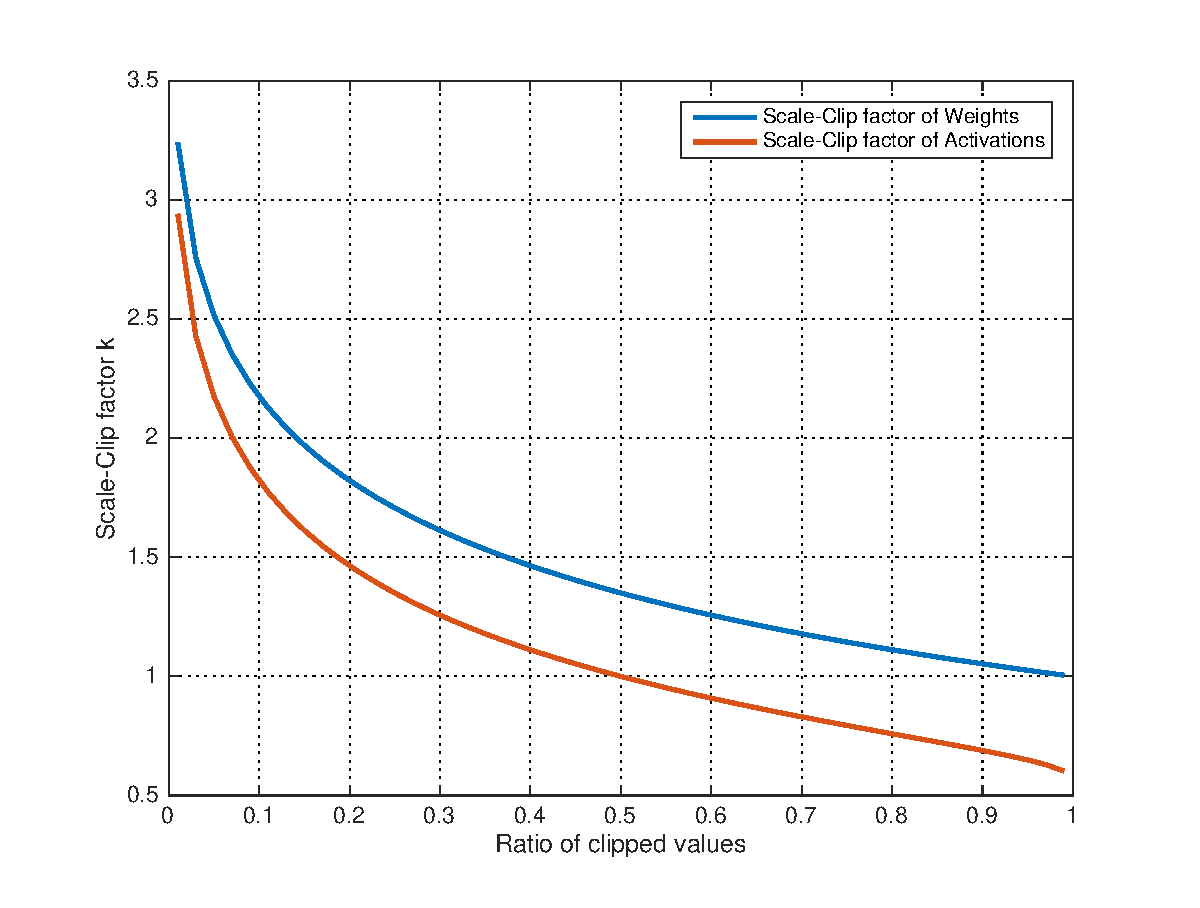
\includegraphics[width=0.45\textwidth]{scale-factor.eps}
	\caption{Relationship between Proportion of clipped values and Scale Clip factor $k$.}\label{fig:scale-factor}
\end{figure}

% To estimate this ratio, we simplify the training process as a we first consider about weights. We approximate the trajectory of weights during the training process as a brownian motion. When Scale-Clip method is utilized in the training process, the brownian motion turn to be a brownian motion with boundary.

% As we know, a standard brownian motion without boundary condition results in a Gaussian Distribution. However, the distribution a brownian motion with boundary condition depends on the way that particles interact with the boundary. 

% \paragraph{Absorption boundary} When weights hit the clipping threshold $\alpha$, they keep still at the boundary, which is called direct clipping. The clipping function is shown as below. 
% \begin{equation}
% Q(w)=\left\{
%    \begin{array}{lr}
%       \alpha, & w \ge \alpha \\
%       w, & w \in (-\alpha, \alpha) \\
%       -\alpha, & w \le -\alpha 
%    \end{array}
% \right.
% \end{equation}


% This boundary will lead all weights in brownian motion converge at the boundary when the time $t$ is large enough.  


% \paragraph{Reflective boundary} This boundary force all weights hitting the threshold to ``turn back'', which is called reflective clipping. The function is written as below. 
% \begin{equation}
% Q(w)=\left\{
%    \begin{array}{lr}
%       Q(2\alpha - w), & w \ge \alpha \\
%       w, & w \in (-\alpha, \alpha) \\
%       Q(-2\alpha - w), & w \le -\alpha 
%    \end{array}
% \right.
% \end{equation}
% With this boundary condition, the distribution will converge to a uniform distribution when the time $t$ goes infinity. 
For activation, we replace all vanilla ReLU layers with our Scale-Clip ReLU layers.
Different from determining the threshold directly as (\ref{threshold}), the mean of activations depends on the input data. We use \textbf{E}xponential \textbf{M}oving \textbf{A}verage (EMA) to estimate the mean of activation similar as \cite{jacob2017quantization}. 
\begin{equation}
\begin{aligned}
	T^{a}_{i}(t) & = k \cdot \text{EMA}^{t}(|\mathbf{A}_{i}|)) \\
    & = k \cdot (\mu \mathbb{E}(\mathbf{A}_{i}) + (1-\mu)\text{EMA}^{t-1}(|\mathbf{A_i}|)) \\
    & = \mu k\mathbb{E}(\mathbf{A}_{i}) + (1-\mu)T^{a}_{i}(t-1)
\end{aligned}
\end{equation}
where $\mu \in (0, 1)$. The EMA algorithm introduces a fluctuation of threshold when we train the model with Scale-Clip ReLU layer. So a small $\mu$ is used in our implementation. 

Different from weights, the vanilla ReLU layer clips input values by zero. We also assume the original input data follow Gaussian Distribution, then the relationship between proportion of clipped numbers and $k$ can be obtained in the same way. Here $\text{cdf}(x)=\frac{1}{2}\left[1+\text{erf}(\frac{x}{\sigma \sqrt{2}})\right]$.
\begin{equation}
k(\frac{1}{\sqrt{2\pi}\sigma}\int_{0}^{
T^a}xe^{-\frac{x^2}{2\sigma^2}}dx + T^a(1-\text{cdf}(T^a))=T^a
\label{eq:activation}
\end{equation}
% which indicating $k$ can be small than the Scale-Clip of weights.
It can be seen that similar relationship are shared with the Scale-Clip factor of weights. So a same scheme is utilized for select the Scale-Clip factor of activations.
% During training process, the distribution gradually transitions from Gaussian to the steady-state distribution of brownian motion, Under the assumption that the initial weights follow Gaussian Distribution, we can regard the distribution of trained weights as the intermediate result between Gaussian Distribution and the two kinds of steady-state distributions. which is an important guidance for choosing the value of $k$. In fact, we can set $k$ between the $\frac{\max{|\mathbf{W}_i|}}{\overline{|\mathbf{W}_{i}|}}$ of steady-state distributions and Gaussian distribution. With this , the range of a proper $k$ is estimated as $(2, 3\sqrt{\frac{\pi}{2}})$.
Our training process with Scale-Clip is shown in following Algorithm \ref{alg:1}.
\begin{algorithm}[!ht]
	\caption{Process of Training Float Point Model with Scale-Clip}\label{alg:1}
	\begin{algorithmic}[1]
		\Require input data, CNN architecture,$k$
		\Ensure trained float point model
		\State initiate the CNN model
		\For{$epoch$}
        \For{ each Layer}
        \State calculate the threshold of Scale-Clip with $T^w_{i}=k \cdot \mathbb{E}{|\mathbf{W}_{i}|}$ and $T^a_{i}=k \cdot \mathbb{E}{|\mathbf{A}_{i}|}$
		\State clip the $W_i$ with $T^w_i$
        \State clip the $A_i$ with $T^a_i$
		
        
        \EndFor
		\State forward \& backward 
		\For{ each Layer $W_i$}
		\State update the weight
		\EndFor	
		\EndFor
		\State \Return float point model
	\end{algorithmic}
\end{algorithm}

% \section{Extension and Framework}\

% In this section, we generalize the Scale-Clip method from quantizing weight to quantizing activation,
% and then we assemble these Scale-Clip methods into quantization framework to get final fixed point model.

% \subsection{Extensive Discussion to Activation}\

% Since each layer's output is composed of two parts: weight and input activation, 
% the quantized loss is also sourced from not only weight but also input activation.
% In addition, we quantize activation with the same way as quantizing weight in the quantization process.
% Similar to Theorem \ref{the:range-mean}, we have conlusion that if input has smaller $\frac{\max(|\mathbf{I}_{i}|)}{\overline{|\mathbf{I}_{i}|}}$, there will be also smaller signal loss ratio after quantization.
% So we attempt to shape the distribution of input with Scale-Clip method.

% Thankfully, we observe that the output of $ReLU$ layer is the input of $Conv$ layer, 
% thus we substitude the commen ReLU layer with our Scale-Clip ReLU layer.
% Different from determining the threshold directly as (\ref{threshold}), the mean of activations depends on the input data. Similar as [Google], we use exponential moving average to estimate the mean of activation. Take $i$th layer as an example.
% \begin{equation}
% \begin{aligned}
% T_{i}^{t} & = k \cdot EMA^{t}(|\mathbf{I}_i|)) \\
% & = k \cdot (\alpha |\overline{\mathbf{I}_i}| + (1-\alpha)EMA^{t-1}(|\mathbf{I}_i|)) \\
% & = \alpha k|\overline{\mathbf{I}_i}| + (1-\alpha)T_{i}^{t-1}
% \end{aligned}
% \end{equation}
% where $\alpha \in (0, 1)$. The EMA algorithm introduces a fluctuation of threshold when we train the model with Scale-Clip method. So a small $\alpha$ is used in our implementation. 

% Here we provide a simple method to implement the $Scale-Clip$ $ReLU$ with following form: 
% \begin{equation}
% 	\min_{T_{i}}||T_i-k*\overline{\mathbf{I}_i}||_{2}^{2}
% \end{equation}
% update the $T_{i}$ with
% \begin{equation}
% \begin{aligned}
% 	T_{i}
% 	&=T_{i}-\lambda \cdot \triangledown T_{i}\\
% 	&=T_{i}-\lambda \cdot (T_i-k*\overline{\mathbf{I}_i})
% \end{aligned}
% \end{equation}

\section{Experimental Results}
In this section, we evaluate our method and framework by conducting extensive quantization experiments. We first demonstrate that Scale-Clip method helps to shape the weight distribution of full precision network into a distribution suitable for quantization. Then we report our quantization result on a ImageNet classification task and compare it with other low bit quantization work. We also demonstrate that our Scale-Clip method can be generalized to other tasks, such as detection and semantic segmentation. We implement our Scale-Clip Net by PyTorch framework.
\subsection{Analysis of Scale-Clip Method}\label{an illustrating example}
To analysis the versatility of Scale-Clip Method, we examine the effect of Scale-Clip algorithm in different quantization settings.

\subsubsection{Experiment Settings}
We choose a simple network, ResNet18, and train it on CIFAR-100. We set mini batch size as 64, and our learning rate is 0.1. The number of epochs is set as 150, except for 5 warm-up epochs. SGD is used for optimizing the parameters, with the momentum as 0.9 and weight decay as 0.0005. Besides, we apply Scale-Clip method on all regular convolution layers. And Scale-Clip factor $k$s are tested to show the its effect to the model. In our experiments,  we set $k$ as 2, 2.5, 3, 4 and $\infty$ according to the recommended range mentioned before. To be mentioned, as the Scale-Clip factor $k$ goes infinity, the Scale-Clip Net comes down to a regular network.

\subsubsection{Result} We compare the distributions of weights trained in different Scale-Clip factors. Fig~\ref{fig:scale-factor} shows the how different $k$s shape the distribution of trained weights. The distribution of regular convolution weights produce a distribution similar to a Gaussian, with most of data lying around central part but some resting in its tail. When $k$ gets smaller, outliers of distribution are removed, resulting a flat distribution. When $k$ is 2.5 or 2, however, the range narrows, and two peaks start emerging at the clipping boundaries, forming a distribution similar to Ternary Distribution.  

\begin{figure}[ht!]
	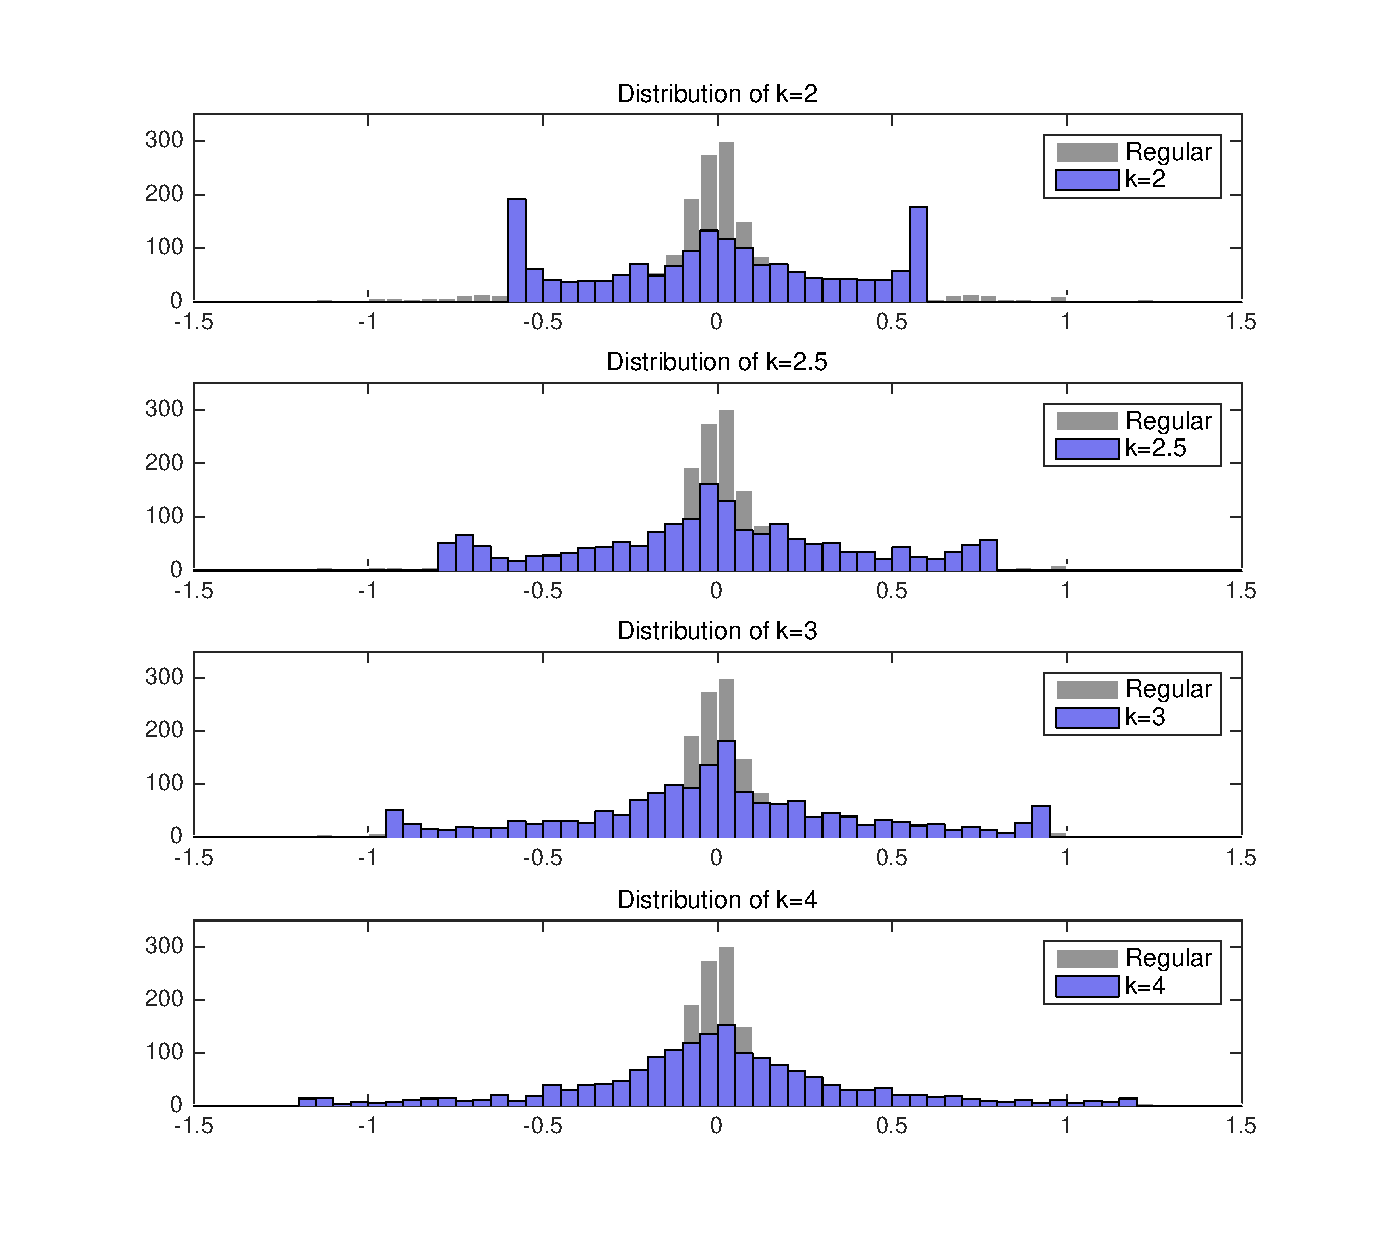
\includegraphics[width=0.45\textwidth]{dist4.eps}
	\caption{Weight distribution of different Scale-Clip factor. For comparison, the background is the distribution of weights trained without Scale-Clip}\label{cifar100_distribution}
\end{figure}

Fig~\ref{fig:qwlr} plots the curves of quantization bit number vs. QLR in different Scale-Clip $k$. It can be observed that the curve of regular convolution settings($k=\infty$) is above other curves and with smaller Scale-Clip factor, the QLR is consistently lower than the lager Scale-Clip factor in all quantization bit numbers. This indicates that training with Scale-Clip method can alleviate the QLR to a great extent, especially in low bit, so that a higher quantization performance can be expected. 

\begin{figure}[ht!]
	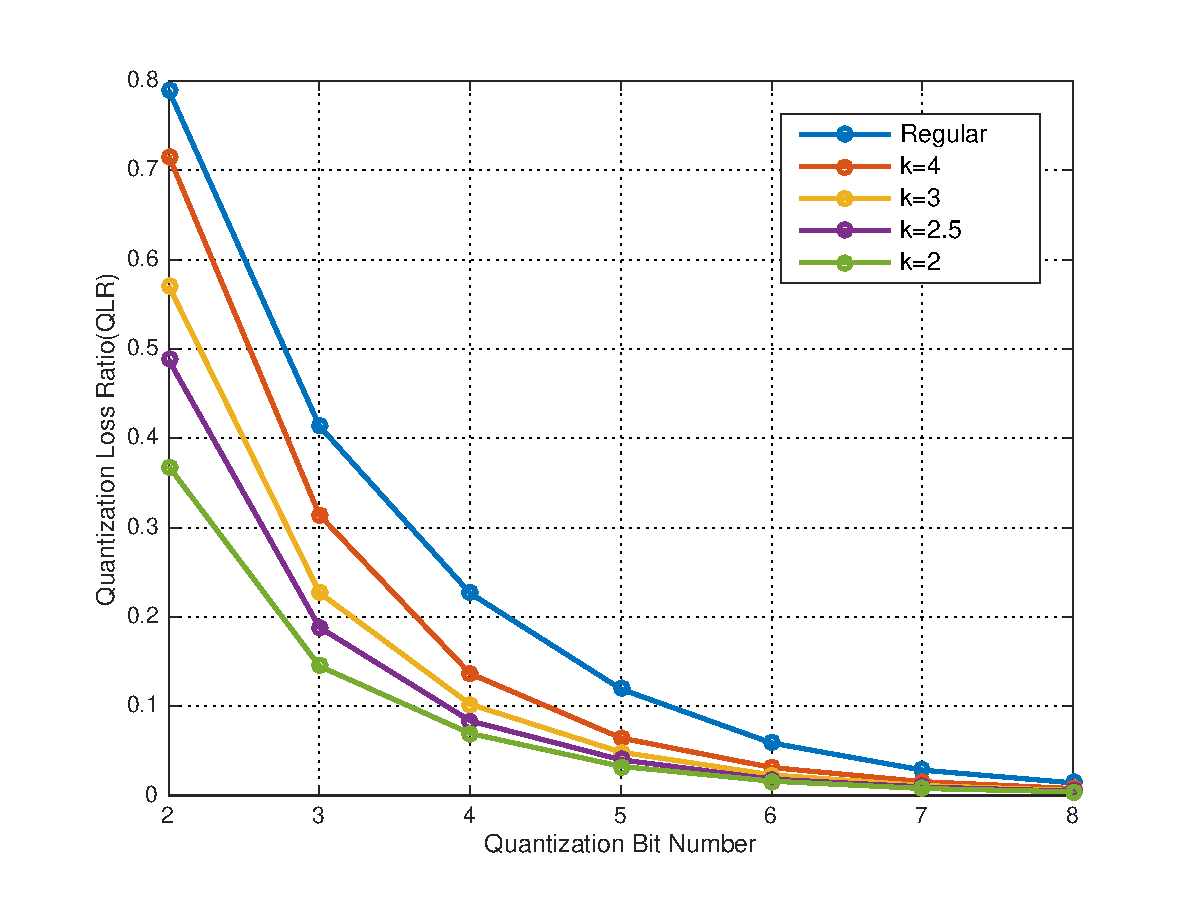
\includegraphics[width=0.45\textwidth]{qlr.eps}
	\caption{Loss Ratio After Quantizing First Layer's weights. The Regular curve is the QLR trained without Scale-Clip.}\label{fig:qwlr}
\end{figure}

We show the accuracy of different $k$ settings in Fig~\ref{fig:diffk}. First, the results of full precision model show that if we decrease $k$, the performance of the model will gets worse. This is because Scale-Clip restricts the distribution of weights and impairs the network performance. However, only a fraction of weights are clipped as our $k$s lie in the recommended range, the accuracy merely drops from the best result within 1\%. As for quantization performance, We quantize the weights of trained model from 2 to 8 bits, with activations as full precision. Results shows the model quantized in relatively large bits only suffer a little performance degradation. As the Scale-Clip factor decreases, the degradation becomes negligible, which is in accordance with the relationship between QLR and $k$. Moreover, lower Scale-Clip factors show their advantages in extremely low bit quantization scenario. We can see that the performance of 2/3bit quantization in $k=\{2,2.5\}$ surpasses larger $k$'s counterpart with over 4\%. The results reflect the effectiveness of Scale-Clip for its capability of make the distribution of weight more suitable for low bit quantization.

\begin{figure}[ht!]
	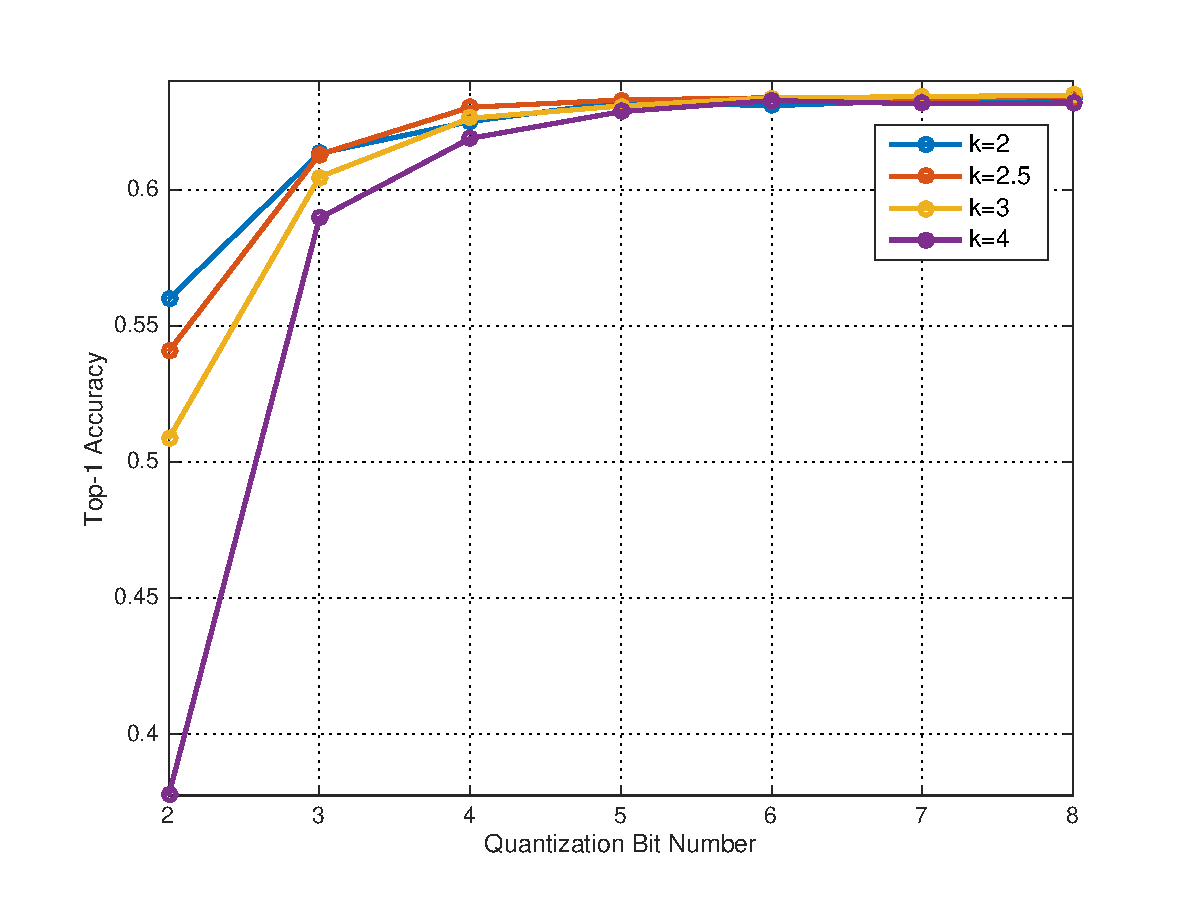
\includegraphics[width=0.45\textwidth]{acc.eps}
	\caption{Top-1 Accuracy of different Scale-Clip factors.}\label{fig:diffk}
\end{figure}
% We expect that QLR and the distribution of 
% .  We can see a sharp peak at the clipping boundary when $k$ is small. 
% \subsubsection{Analysis of QLR}
% \subsubsection{Analysis of Distribution}


% In Fig \ref{cifar100_distribution}.
% we show the first layer's weight distributions of Model \uppercase\expandafter{\romannumeral1} and Model \uppercase\expandafter{\romannumeral2} after training 150 epochs. 
% From the figure, we find the weight distribution of Model \uppercase\expandafter{\romannumeral1} similar to a Gaussian Distribution while comparing to Model \uppercase\expandafter{\romannumeral1}, Model \uppercase\expandafter{\romannumeral2} has a flatter distribution with two spikes at the clipping boundary. 


% Then we quantize the weights and activations of Model \uppercase\expandafter{\romannumeral1} and Model \uppercase\expandafter{\romannumeral2} 
% both from 1 bit to 8 bit. Notice that we just quantize the convolution layers without fine-tuning.
% Fig~\ref{fig:qwlr}, we shows the $\text{QLR}_{1}$  of first layer of Model \uppercase\expandafter{\romannumeral1} and Model \uppercase\expandafter{\romannumeral2} in different quantization bits. It can be observed that when bit number  gets lower, the $\text{QLR}_{1}$  rapidly increases. Applying Scale-Clip method, however, alleviate the quantization loss to a great extent, especially in low bit.
% Fig \ref{quantized_result} shows the Top-1 and Top-5 of quantized Model \uppercase\expandafter{\romannumeral1} and Model \uppercase\expandafter{\romannumeral2} accuracy on testing images. We can observe that at relatively large quantization bits, two models have similar performance. In the smaller quantization bits case, however, compared to Model \uppercase\expandafter{\romannumeral1}, 
% Model \uppercase\expandafter{\romannumeral2} gets better results, indicating that the smaller $\text{QLR}_{i}$ helps maintain the performance and our Scale-Clip method is favorable for the quantization, especially in low bit case.


% \begin{figure}[ht!]
% 	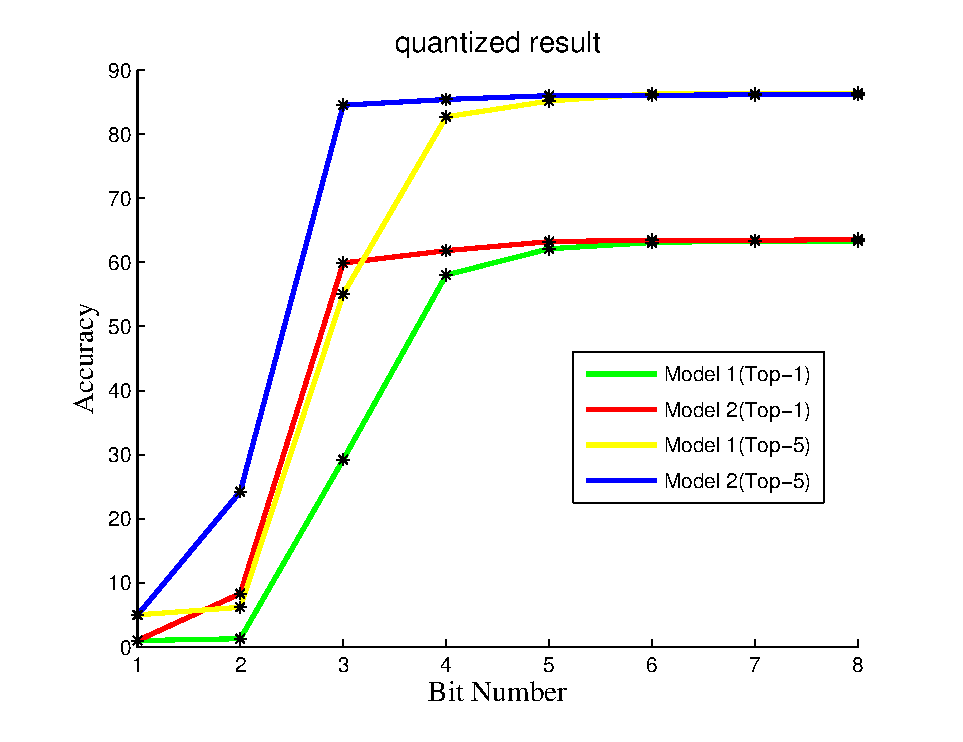
\includegraphics[width=0.45\textwidth]{quantized_result.eps}
% 	\caption{Test Accuracy of Quantized Model \uppercase\expandafter{\romannumeral1} and Model \uppercase\expandafter{\romannumeral2}.}\label{quantized_result}
% \end{figure}
% Thus according to above results, we conclude that Scale-Clip method can shape the weight distribution of float point model into a suitable one for quantization,
% and make the quantized model outperform than the original method.
% \subsection{Effect of Scale Clip factor $k$}
% To fully understand the effect of different Scale Clip factor $k$, we train a ResNet18 model on CIFAR-100 with different Scale-Clip factor settings. We compare the accuracy, the weight distributions and quantization results of different $k$, and show how $k$ effects the model quantization performance.
% \begin{figure}[ht!]
% 	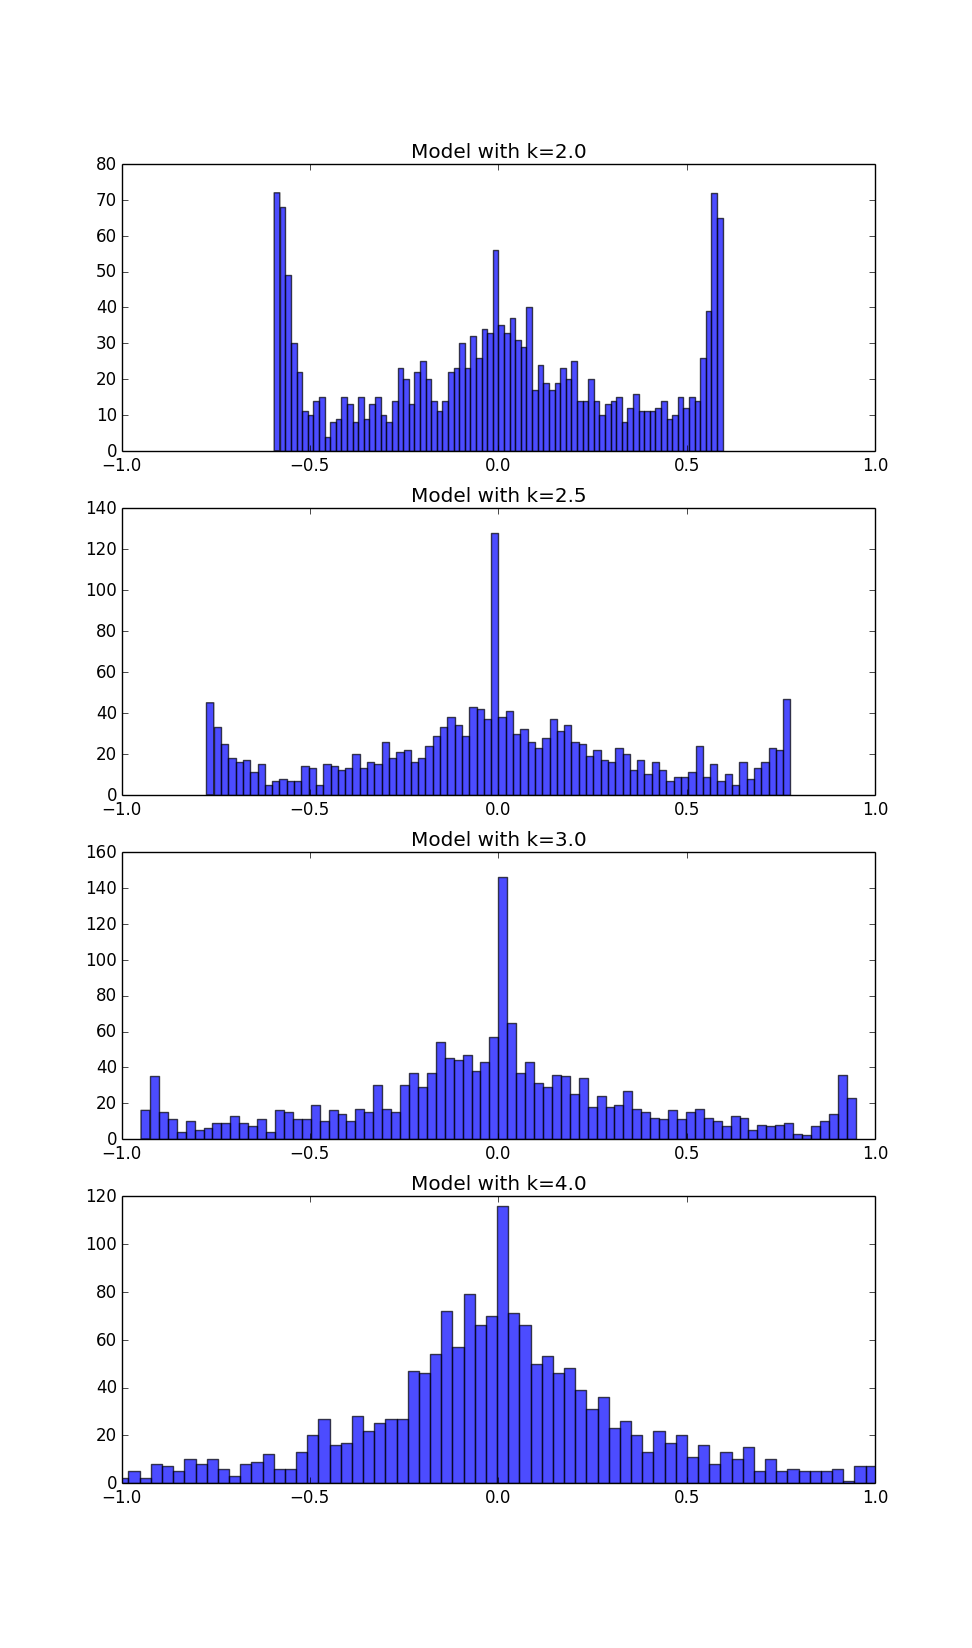
\includegraphics[width=0.45\textwidth]{dist4.png}
% 	\caption{Distribution result with different Scale-Clip factor $k$.}\label{fig:scale-factor}
% \end{figure}
% Fig~\ref{fig:scale-factor} shows the how different $k$ shape the distribution of trained weights. We can see a sharp peak at the clipping boundary when $k$ is small. 
% Table~\ref{tab:diffk} shows the relationship between accuracy and Scale Clip factor. It can be observed that small $k$ impair the network performance, as the proportion of clipped values increases which has been analyzed above. We then quantize all weights of model in different numbers of bits and plot the performance with and without finetuning in Fig. We can find that although in small $k$ settings, the performance of full precision model is getting poor, the quantization performance in extremely low bit (e.g 2bit/3bit) is slightly better than the counterpart of larger $k$ settings. This indicates the select 

% \begin{table}
% 	\caption{Accuracy of different $k$ and different quantization bit number without finetuning}
%     \label{tab:diffk}
% 	\begin{tabular}{ccccccccc}
% 		\hline
% 		bit  & 2 & 3 & 4 & 5 & 6 & 7 & 8 & f\\
% 		\hline
% 		k=2 &55.98&61.34&62.51 & 63.23 & 63.09 & 63.28 &63.33&63.33 \\
% 		k=2.5 &54.06&61.3&63.03 & 63.3 & 63.38 & 63.33 & 63.45&63.47 \\
%         k=3  &50.86&60.47&62.63& 63.08 & 63.38 & 63.42 & 63.48&63.51 \\
%         k=4  &37.75&58.96&61.89& 62.87 & 63.28 & 63.16 &63.19&63.16 \\
% 		\hline
% 	\end{tabular}
% \end{table}

\subsection{Quantization On ImageNet}
\paragraph{ImageNet} 
ImageNet dataset has about 1.2 million training images and 50 thousand validation images. 
Each image is annotated as one of 1000 object classes.
The size of each image is $256\times 256$, and we crop the training image by $224\times 224$ as input image,
and use the center crops of validation image to validate the model.
\paragraph{ResNet50}
ResNets50 has batch normalization layers and relief the vanishing gradient problem by using shortcut connections.
Compared to ResNet18, ResNet50 has $1\times1$ convolution layers.
In the training process of full precision model, 
we substitute the ReLU layers with our Scale-Clip ReLU layers, and set the scale clip factor as $6$.
We also use the Scale-Clip for weights and set the scale clip factor as $2$.
In the training settings, the learning rate is 0.1, batch size is 64, maximal epoch number is 150,
the weight decay is 0.0005, and the momentum is 0.9.
We use the SGD method to optimize the model.
\paragraph{Results}
We quantize the convolutional layers' weight and input activation with the combination of (2, 8) and (4, 4)bit.
In the fine-tuning step, the learning rate starts at 0.001 and is divided by 10 every 20 epochs, 
the batch size is 64, the weight decay is 0.0005, and the momentum is 0.9.
In the inference process, we fix the threshold of the Scale-Clip ReLU layers and remove all Scale-Clip operations.

We choose the best accuracy in fine tuning process to compare with some open benchmarks reported from SYQ\cite{faraone2018syq}, FGQ\cite{mellempudi2017ternary} and DoreFa-Net\cite{zhou2016dorefa}, which are the sate-of-the-art methods.
The results are illustrated in Table 
\iffalse
\begin{table}
	\caption{Accuracy Comparison with [2,4]}
	\begin{tabular}{|c|l|l|l|l|}
		\hline
		\diagbox{Model}{Accu}{bit}  &  Top-1 & full prec & Top-5 & full prec\\
		\hline
		SYQ         &    70.9       & - & 88.6 & - \\
		FGQ          &    68.6            & - & 88.6 & - \\
		DereFa-Net    &    68.6     & - & 86.6 & - \\
		\hline
		Ours(k=2)    &    70.8      & 75.2 & 89.9 & 92.4 \\
		Ours(k=2,6)   &    -     &  74.8  &     &  \\
		\hline
	\end{tabular}
\end{table}
\fi
\begin{table}
	\caption{Accuracy Comparison with [4,4]}\label{ta:imagenet_4_4}
	\begin{tabular}{|c|l|l|l|l|}
		\hline
		\diagbox{Model}{Accu}{Bits}  &  Top-1 & full prec & Top-5 & full prec\\
		\hline
		DoReFa-Net    &    71.4     & - & 86.6 & - \\
		\hline
		Ours(k=2,6)   &    72.7     &  74.7  & 90.9   & 92.1 \\
		\hline
	\end{tabular}
\end{table}
\begin{table}
	\caption{Accuracy Comparison with [2,8]}\label{ta:imagenet_2_8}
	\begin{tabular}{|c|l|l|l|l|}
		\hline
		\diagbox{Model}{Accu}{Bits}  &  Top-1 & full prec & Top-5 & full prec\\
		\hline
		SYQ         &    72.6       & 76 & 90.6 & 93 \\
		FGQ          &    70.8            & - & - & - \\
		DoReFa-Net    &    68.6     & - & 90.6 & - \\
		\hline
		Ours(k=2,6)   &    73.6     &  74.7  & 91.6    & 92.1 \\
		\hline
	\end{tabular}
\end{table}
From Table \ref{ta:imagenet_4_4} and Table \ref{ta:imagenet_2_8}, although the performance of full precision model which adds our Scale-Clip method is not good as other full precision model, the final low-bit model outperforms that these methods more than $1\%$. 

% \subsection{Detection On PASCAL-VOC}
% We validate Scale-Clip Algorithm on PASCAL-VOC dataset to evaluate the effect of our quantization method on detection tasks. We choose Faster-RCNN with ResNet-50 backbone, a popular detection architecture as baseline model. Both quantization result and fine-tuning result based on quantization model will be reported.

% \paragraph{Faster-RCNN with ResNet-50}
% Different from classification models above, Faster-RCNN is composed of Region Proposal Network, RoI-pooling, Bounding Box Regression and other modules, where more complex operations are involved so that quantization cannot be well defined every where. Also, we keep Bounding Box Regression as full precision for a more precise regression result. So in our experiment, only convolution layers are quantized and all ReLU layers are replaced as Scale-Clip ReLU. As for the training settings, a ImageNet pretrained model is used to initialize the ResNet-50 backbone. For PASCAL-VOC, We set the learning rate as 0.1, batch size as 8, epoch number as 50 except for 5 warm-up epochs, the weight decay as 0.0005, the momentum as 0.9. As for fine-tuning step, we set the learning rate as 0.0001, epoch number as 10, and other hyper parameters as the same as their training settings. 

% \paragraph{Results}
% Like results in classification, different quantization bits and $k$ for Scale-Clip are explored. We keep the input image as 8bit throughout the experiment. Even through the detection task is more difficult than classification, we can observe a good quantization  performance of Scale-Clip method. Notice that without finetuning, there is only a little decrease in mAP. Except for $(2, 4)$, there is only a slight loss within 1\% in other quantization settings, indicating that our Scale-Clip method can well maintain the performance after quantization. We compare our result with Weighted Entropy Loss. It can be observed that after finetuning, our mAP results is consistently better than other work at different quantization bits, demonstrating that our quantization method can be generalized to detection task and better than other quantization methods.

\begin{table}
	\caption{mAP of PASCAL-VOC. `f' respects to utilizing finetuning. Notice that activations are not quantized in \cite{yin2016quantization}}
    \label{tab:map}
	\begin{tabular*}{8.5cm}{cccccc}
		\hline
		Model   & float &  (8,8) & (4,8) & (4,4) & (2,4)  \\
		\hline
		Ours(k=3)   & 79.0 &  78.7  & 78.8 & 78.1 & 73.2\\
		Ours(k=3)+f & 79.0 & -  & - & 79.0 & 78.3\\
        \hline
        Park et al.\shortcite{park2017weighted}   & 77.61 & 73  & 66 & - & - \\
        Yin et al.\shortcite{yin2016quantization} & 77.46 & - & 74.37 & - & - \\
		\hline
	\end{tabular*}
\end{table}

% \subsection{Segmentation On Cityscape}
% To better examine the generality of Scale-Clip method, We perform image segmentation on Cityscape dataset. We test Scale-Clip method on a image segmentation architecture, PSPNet with ResNet-50 backbone. And both quantization result and fine-tuning result based on quantization model will be reported.

% \paragraph{PSPNet with ResNet-50}
% We replace all regular convolution layers and ReLU layers in PSPNet as the Scale-Clip version. As for the training settings, we train from a ImageNet pretrained model. We set the learning rate as 0.01, batch size as 8, epoch number as 500 except for 5 warm-up epochs, the weight decay as 0.0005, the momentum as 0.9. As for fine-tuning step, we set the learning rate as 0.0001, epoch number as 50, and other hyper parameters as the same as their training settings. 

% \paragraph{Results}
% Like results shown above, we test our Scale-Clip on   different quantization bits for Scale-Clip. Input images are set as 8 bit throughout the experiment. From the results shown in Table , it can be found that after finetuning, the mIoU results in all quantization bit settings only suffer a negligible decrease, even in the extremely low bits. However, for the quantization performance without finetuning, we observe a drop from full precision model (around 3-10\%). We believe that the reason is the difficulty of fitting segmentation results on Cityscape causing the trained network more sensitive to quantization noise. In summary, our Scale-Clip method can also achieve a good performance in segmentation task. 

\begin{table}
	\caption{mIoU of Cityscape, `f' respects to utilizing finetuning.}
    \label{tab:miou}
	\begin{tabular}{cccccc}
		\hline
		Model  & float  &  (8,8) & (4,8) & (4,4) & (2,4) \\
		\hline
        Ours(k=3)  & 75.6 & 75.31  & 72.48 & 68.5 & 38.24 \\
        Ours(k=3)+f & 75.6 & 75.66 & 75.29 & 75.62 & 74.7 \\
		\hline
	\end{tabular}
\end{table}

\subsection{Versatility of Scale Clip}
To demonstrate the versatility, we validate Scale-Clip method on other more complex computer vision task. We perform object detection on PASCAL-VOC dataset and Semantic Segmentation on Cityscape dataset. Both quantization result and finetuning result based on quantization model will be reported. 

\subsubsection{Detection on PASCAL-VOC}
We choose Faster-RCNN with ResNet-50 backbone, a popular detection architecture as the baseline model.
Different from classification models above, Faster-RCNN is composed of Region Proposal Network, RoI-pooling, Bounding Box Regression and other modules, where more complex operations are involved so that quantization cannot be well defined every where. Also, we keep Bounding Box Regression as full precision for a more precise regression result. So in our experiment, only convolution layers are quantized and all ReLU layers are replaced as Scale-Clip ReLU. As for the training settings, a ImageNet pretrained model is used to initialize the ResNet-50 backbone. For PASCAL-VOC, We set the learning rate as 0.1, batch size as 8, epoch number as 50 except for 5 warm-up epochs, the weight decay as 0.0005, the momentum as 0.9. As for fine-tuning step, we set the learning rate as 0.0001, epoch number as 10, and other hyper parameters as the same as their training settings.

\subsubsection{Segmentation on Cityscape}
We test Scale-Clip method on the image segmentation network, PSPNet with ResNet-50 backbone.
We replace all regular convolution layers and ReLU layers in PSPNet as the Scale-Clip version. As for the training settings, we train from a ImageNet pretrained model. We set the learning rate as 0.01, batch size as 8, epoch number as 500 except for 5 warm-up epochs, the weight decay as 0.0005, the momentum as 0.9. As for fine-tuning step, we set the learning rate as 0.0001, epoch number as 50, and other hyper parameters as the same as their training settings. 

\subsubsection{Result}
Like experiments in classification, we keep the input image as 8bit throughout the experiment and test different quantization bits. Under the consideration of complexity of these two tasks, the Scale-Clip factor $k$ is set as 3 for both weights and activations in order to avoid chopping off too many values. Even through the detection and semantic segmentation tasks are more difficult than classification, we can observe a good quantization  performance after utilizing Scale-Clip method. 
From Table~\ref{tab:map}, we can notice that without finetuning, there is only a little degradation in mAP. As for semantic segmentation, Table~\ref{tab:miou} also presents a similar result, with the maximum degradation within 7\%, except for 2bit weights and 4bit activations(2,4). 
% This indicates that our Scale-Clip method maintains its effectiveness when transferring to more complex tasks. On the other hand, 
Due to the large $k$, there appears a non-negligible performance drop in (4,4) and (2,4) quantization. We believe that the reason is the difficulty of fitting segmentation results on Cityscape causing the trained network more sensitive to quantization noise.
However, after finetuning based on the quantized model, the performances on both tasks are retrieved, with a drop from full precision model within 1\%, even in the (4,4) and (2,4) cases. We compare our quantized detection results with \cite{park2017weighted} and \cite{yin2016quantization}. Notice that the network architectures tested in \cite{park2017weighted} and \cite{yin2016quantization} are R-FCN, a modified version of Faster-RCNN, slightly different from ours. Also, the quantization schemes utilized are both non-uniform. Despite of the small differences, it can be observed that after finetuning, our mAP results is consistently better than other work at different quantization bits. As for semantic segmentation, however, as far as we know, there is no quantization benchmark of segmentation result on large datasets, especially in low bit quantization. Our segmentation quantization result with 2bit weights and 4bit activations only drops 0.7\% compared to the full precision model, demonstrating that our quantization method can be generalized to detection task and better than other quantization methods. In summary, the experiments prove that our Scale-Clip method can be generalized to other tasks without losing its effectiveness. 

% \subsection{Quantization without finetuning}
% We compare the quantization result 
% Notice that without finetuning, there is only a little decrease in mAP. Except for $(2, 4)$, there is only a slight loss within 1\% in other quantization settings, indicating that our Scale-Clip method can well maintain the performance after quantization. 



\section{Conclusion}
In this paper, we start from SNR and analyze the relationship between the model distribution and the quantization performance decreases. We present a ratio called QLR to describe the quantization loss, and prove that it is proportional to the ratio of abs-max to abs-mean. To minimize the QLR and improve quantization performance, we propose a novel approach called Scale-Clip to make the weights and activations converge to a distribution suitable for quantization. We further discuss the trade-off between minimizing the QLR and the loss of information caused by Scale-Clip method, and offer a reasonable range of Scale Clip factor $k$. Then we incorporate Scale Clip method into regular convolution and ReLU layers and design the quantization training framework. We demonstrate our method on several kinds of tasks, comparing the quantization performances with and without fine-tuning. We quantize models of different architectures and achieve only with 1\% loss in performance with low bit weights (2bit/4bit) and activations (4bit). We highlight our approach can not only outperform than other state-of-the-art low bit quantization work, but can also be generalized to many common computer vision tasks. Further research includes analyzing how robust a network is to quantization error and how to adaptively set the Scale-Clip factor $k$ without specifically tuning by hand.

% In this work, we considered the problem of training high
% performance deep networks with low-precision. This was
% achieved by designing two approximators for the ReLU
% non-linearity. The first is a half-wave Gaussian quantizer,
% applicable in the feedforward network computations. The
% second is a piece-wise continuous function, to be used in
% the back propagation step during learning. This design overcomes
% the learning inefficiency of the popular binary quantization
% procedure, which produces a similar approximation
% for the less effective hyperbolic tangent nonlinearity.
% To minimize the problem of gradient mismatch, we have
% studied several backwards approximation functions. It was
% shown that the mismatch is most affected by activation outliers.
% Insights from the robust estimation literature were
% then used to propose the clipped ReLU and log tailed ReLU approximators. The network that results from the combination
% of these with the HWGQ, denoted HWGQ-Net was
% shown to significantly outperform previous efforts at deep
% learning with low precision, substantially reducing the gap between the low-precision and full-precision various state of-the-art
% networks. These promising experimental results
% suggest that the HWGQ-Net can be very useful for the deployment
% of state-of-the-art neural networks in real world
% applications
\bibliography{ref}
\bibliographystyle{aaai}
\end{document}
